% =============================================================================
% Chapter 3 — Methods: The QRC-EV System
% =============================================================================

\chapter{Methods: The QRC-EV System}
\label{chap:methods}

This chapter describes the QRC-EV system in detail. We begin with the
GPU-accelerated quantum reservoir (\S\ref{sec:gpu_reservoir}), then the
QHMM-OOM representation and OMLE training (\S\ref{sec:qhmm_oom_impl}),
the TD($\lambda$) eligibility trace mechanism (\S\ref{sec:td_lambda_impl}),
the optimistic planning module (\S\ref{sec:optimistic_impl}), and finally
the complete end-to-end pipeline (\S\ref{sec:pipeline}).

% =============================================================================
% §3.1  GPU-Accelerated Quantum Reservoir
% =============================================================================

\section{GPU Quantum Reservoir}
\label{sec:gpu_reservoir}

\index{GPU reservoir}
\index{CUDA Quantum}
\index{Amazon Braket}

The reservoir is implemented using NVIDIA's CUDA Quantum platform
\citep{nvidiacudaq} integrated with Amazon Braket
\citep{amazonbraket}. This provides GPU-accelerated simulation of the
quantum register without the overhead of physical quantum hardware access,
while remaining compatible with actual quantum processors through the
Braket API.

\index{NVIDIA CUDA Quantum}
\index{Amazon Braket}

\subsection{State Representation}

\index{quantum state!statevector}
The $n$-qubit register is represented as a statevector
$\ket{\psi} \in \mathbb{C}^{2^n}$ using the full complex amplitude
representation. The state is stored as a PyTorch tensor on GPU
(\verb|torch.complex128|) and updated in place using sparse gate
operations.

\index{sparse gates}
\index{quantum gates!single-qubit}
\index{quantum gates!ZZ}

Single-qubit gates are applied via \verb|torch.einsum| contracts with
the appropriate qubit axis, avoiding full matrix multiplication on the
$2^n$-dimensional space. Two-qubit ZZ interactions
$U_{ZZ}(\theta) = e^{-i\theta Z\otimes Z}$ are applied using sparse
bit-mask operations: the phase $e^{-i\theta}$ or $e^{i\theta}$ is
multiplied into the state entries corresponding to the relevant
computational basis states. This gives $\mathcal{O}(2^n)$ complexity per
gate while only storing the state vector in memory.

\index{ZZ interaction}

\subsection{Input Encoding}

\index{input encoding!angle}
\index{parametric gates}
An input vector $u_t \in \mathbb{R}^{d_{\mathrm{in}}}$ is encoded as a
sequence of single-qubit rotations via the \textbf{input encoding map}
$\mathcal{E}_{\mathrm{in}}: \mathbb{R}^{d_{\mathrm{in}}} \to
\{\text{unitary on } \mathbb{C}^{2^n}\}$:

\index{input encoding}
\begin{subequations}
\label{eq:input_encoding}
\begin{align}
\theta_{t,j} &= \bigl( W_{\mathrm{in}} u_t \bigr)_j + b_j,
& j &= 0, \ldots, n-1, \\[4pt]
U_{\mathrm{in}}(u_t) &= \bigotimes_{j=0}^{n-1}
  R_X(\theta_{t,j}) \cdot R_Z(\theta_{t,j}),
\end{align}
\end{subequations}
where $W_{\mathrm{in}} \in \mathbb{R}^{n \times d_{\mathrm{in}}}$ and
$b_j \in \mathbb{R}$ are trainable (but fixed after initialization)
input weights, and $R_X$, $R_Z$ are standard rotation operators.
The encoding map is the same at every timestep, allowing the reservoir
to build up temporal correlations through the dissipative channel rather
than through input-dependent unitary structure.

\index{RX gate}
\index{RZ gate}
\index{input scaling}

To prevent gate saturation for large input magnitudes, we apply an
\textbf{input scaling factor} $\gamma_{\mathrm{input}} = 0.5$:
\begin{equation}
\theta_{t,j} \leftarrow \gamma_{\mathrm{input}} \, \theta_{t,j}.
\end{equation}
This keeps the rotation angles in the linear regime of the qubit
dynamics and prevents the reservoir state from concentrating on a small
subset of the Hilbert space.

\index{input scaling}

\subsection{Reservoir Dynamics}

\index{reservoir dynamics}
\index{dissipative channel}
\index{depolarizing channel}
The reservoir dynamics follow a two-step update per timestep:
\index{reservoir update}
\begin{subequations}
\label{eq:reservoir_update}
\begin{align}
\ket{\psi'_t} &= U_{\mathrm{in}}(u_t) \, \ket{\psi_{t-1}}, \qquad
\text{(unitary encoding)} \tag{3.2a} \\
\rho_t &= (1 - p_{\mathrm{depol}}) \, \ket{\psi'_t}\!\bra{\psi'_t}
          + p_{\mathrm{depol}} \, \frac{I}{2^n},
          \qquad \text{(depolarizing channel)} \tag{3.2b}
\end{align}
\end{subequations}
where $\rho_t$ is the density matrix at output and $p_{\mathrm{depol}}$
is the depolarizing probability (default $p_{\mathrm{depol}} = 0.01$).
The depolarizing channel ensures that information does not accumulate
indefinitely in the register, providing an analog of the leaking rate
$\alpha$ in ESNs and enforcing the quantum echo state property.

\index{depolarizing channel!probability}

The use of a \emph{stateful} reservoir—where $\rho_t$ depends explicitly
on $\rho_{t-1}$ through the depolarizing channel—is critical for
temporal memory. In contrast to stateless reservoir computing
\citep{torre2023memory}, the stateful model can accumulate evidence
over multiple timesteps before producing an output.

\index{stateful reservoir}
\index{stateless reservoir}

\subsection{State Evolution and Sequence Processing}

\index{sequence processing}
\index{state evolution}
The reservoir exposes two primary interfaces:

\begin{itemize}
  \item \verb|evolve_state(x)|: Evolves the internal reservoir state by one
    input $x \in \mathbb{R}^{d_{\mathrm{in}}}$ and returns the output
    density matrix $\rho_t$ (flattened to a $2^n$-dimensional real vector).
  \item \verb|process_sequence(X)|: Processes a full input sequence
    $X \in \mathbb{R}^{T \times d_{\mathrm{in}}}$ by iterating
    \verb|evolve_state| and stacking the outputs.
  \item \verb|process_batch(B, T, d_in)|: Processes a batch of $B$ sequences
    in parallel, using vectorized GPU operations.
\end{itemize}

\index{GPU!batch processing}
\index{PyTorch}

For multi-qubit registers ($n \geq 8$), the batched interface processes
all qubits in a single GPU kernel launch, achieving near-linear
throughput scaling with qubit count on NVIDIA Ampere and Blackwell
architectures.

\index{NVIDIA Blackwell}
\index{RTX PRO 6000}

% =============================================================================
% §3.2  QHMM-OOM Implementation
% =============================================================================

\section{QHMM-OOM Implementation}
\label{sec:qhmm_oom_impl}

\index{QHMM}
\index{OOM!implementation}
\index{OMLE!implementation}

The QHMM-OOM module is implemented in
\verb|src/qrc_ev/agents/qhmm_omle_cudaqx.py|. The implementation follows
the mathematical formalism of Chapter~\ref{chap:background}.

\index{Choi matrix}
\index{Kraus operators}

\subsection{Channel and Instrument Representation}

\index{channel!Choi representation}
\index{instrument!Choi representation}
Every channel $\mathcal{E}_l$ and instrument branch $\Phi^{(a)}_o$ is
stored as a \textbf{Choi matrix} $J(\mathcal{E}_l) \in \mathbb{C}^{S^2 \times S^2}$,
ensuring CPTP constraints can be checked and enforced directly.
The Choi matrix of a channel with Kraus operators $\{K_m\}$ is
\index{Choi matrix!from Kraus}
\begin{equation}
J(\mathcal{E}) = \sum_m \ket{K_m}\!\bra{K_m},
\qquad
\ket{K_m} = (I \otimes K_m) \ket{\Omega},
\end{equation}
where $\ket{\Omega} = \frac{1}{\sqrt{S}} \sum_i \ket{i} \otimes \ket{i}$.

\index{Kraus from Choi}
Conversions between Choi and Kraus representations are provided by:
\verb|choi_from_kraus(Ks)| and \verb|kraus_from_choi(J, S_in, S_out)|.
\index{Kraus!from Choi}

The default initialization uses the \textbf{identity channel}
$K = I$, which gives a valid TP channel with $J_{\mathrm{id}} =
\ket{I}\!\bra{I} / S$ in the normalized convention. This ensures all
initialized channels are physically valid before OMLE training begins.

\index{identity channel}

\subsection{Hilbert-Schmidt Vectorization}

\index{Hilbert-Schmidt!vectorization}
\index{HS vector}
The Hilbert-Schmidt vectorization maps a density matrix $\rho$ to a
real vector $v(\rho) \in \mathbb{R}^{S^2}$ using the orthonormal
matrix-unit basis $\{P_{ij} = \ket{i}\!\bra{j}\}_{i,j=0}^{S-1}$:
\index{matrix-unit basis}
\begin{equation}
v(\rho)[\mu] = \operatorname{tr}[P_\mu^\dagger \, \rho],
\qquad
\rho = \sum_{\mu=0}^{S^2-1} v(\rho)[\mu] \, P_\mu.
\end{equation}
This is implemented as \verb|hs_vectorize(rho, basis)| and
\verb|hs_unvectorize(v, basis)|. The HS representation is real (since
$\operatorname{tr}[P_\mu^\dagger \rho] = \operatorname{tr}[P_\mu \rho]$
is real for Hermitian $P_\mu$ and physical $\rho$), reducing memory
requirements by a factor of 2 relative to the complex density matrix.

\index{HS basis!orthonormal}

The key advantage of the HS representation is that the OOM transition
operators $\{A^{(o,a,o',a')}\}$ are real matrices, enabling efficient
forward and backward passes using standard BLAS operations.

\index{OOM!real operators}

\subsection{Forward Algorithm}

\index{forward algorithm!OOM}
Given a trajectory $\tau = (a_1,o_1, \ldots, a_T,o_T)$, the forward
algorithm computes the sequence of forward messages $\{\alpha_t\}$ and
marginal likelihoods $\{Z_t\}$:
\index{forward message}
\index{marginal likelihood}
\index{unnormalized state}
\begin{subequations}
\label{eq:forward_impl}
\begin{align}
v_0 &= v(\rho_1) \quad \text{(HS vector of initial state)} \\
v_t &= A^{(o_t,a_t,o_{t+1},a_{t+1})} \, v_{t-1}, \qquad t=1,\ldots,T, \\
Z_t &= \mathbf{1}^\top v_t, \qquad
\alpha_t = \frac{v_t}{Z_t}.
\end{align}
\end{subequations}
The forward message $\alpha_t$ satisfies $\sum_\mu \alpha_t[\mu] = 1$
and represents the posterior probability of the hidden state being the
$\mu$-th basis element given the trajectory prefix $\tau_{1:t}$.

\index{forward message!normalization}

The implementation in \verb|OOMModel.compute_forward_backward| computes
$v_t$ and $Z_t$ iteratively, normalizing at each step to avoid numerical
overflow for long trajectories. The log-likelihood is accumulated as
$\sum_t \log Z_t$.

\index{log-likelihood!accumulation}
\index{numerical stability!log-sum-exp}

\subsection{Backward Algorithm and Smoothing}

\index{backward algorithm!OOM}
\index{smoothing}
The backward pass computes $\beta_t$ via the recurrence
\index{backward message}
\index{TD($\lambda$)}
\begin{equation}
\beta_t = \bigl(A^{(o_t,a_t,o_{t+1},a_{t+1})}\bigr)^\top \beta_{t+1}
           \big/ Z_t,
\qquad \beta_T = \mathbf{1},
\end{equation}
where $\bigl(A^{(o,a,o',a')}\bigr)^\top$ is the matrix transpose
(not conjugate transpose) because $A$ is real in the HS basis.

\index{matrix transpose!vs conjugate transpose}

The \textbf{smoothing posterior} is then
\index{smoothing posterior}
\index{forward-backward!smoothing}
\begin{equation}
\xi_t[\mu] = \frac{\alpha_t[\mu] \, \beta_t[\mu]}
                  {\sum_\nu \alpha_t[\nu] \, \beta_t[\nu]} .
\end{equation}
The denominator $\bar Z_t = \sum_\nu \alpha_t[\nu]\beta_t[\nu]$ is a
local model quality metric: if $\bar Z_t \approx 1$, the future is
consistent with the current state estimate; if $\bar Z_t \ll 1$, the
model struggles to explain the observations.

\index{model quality indicator}

The smoothing posterior $\xi_t$ is the basis for all downstream learning:
it provides the state belief that the TD($\lambda$) algorithm uses to
assign credit.

\index{smoothing posterior!usage}

% =============================================================================
% §3.3  TD($\lambda$) Implementation
% =============================================================================

\section{TD($\lambda$) Eligibility Traces Implementation}
\label{sec:td_lambda_impl}

\index{TD($\lambda$)!implementation}
\index{eligibility traces!implementation}

The TD($\lambda$) module is implemented in
\verb|OOMModel.compute_eligibility_traces| and
\verb|OOMModel.update_parameters_from_traces|.

\index{forward trace!implementation}
\index{backward trace!implementation}
\index{combined trace!implementation}

The \textbf{forward trace} is accumulated simultaneously with the forward
pass:
\index{forward trace}
\begin{algorithmic}
\State $e \leftarrow \mathbf{0}_{S^2}$
\For{$t = 0,\ldots,T-1$}
  \State $e \leftarrow \gamma\,\lambda_{\mathrm{fwd}}\,e + \alpha_t$
  \State $e_{\mathrm{forward}}[t] \leftarrow e$
\EndFor
\end{algorithmic}
At each timestep, the current forward message $\alpha_t$ is added to the
decaying trace, implementing the accumulating trace
\citep{sutton2000review}.

\index{accumulating trace}

The \textbf{backward trace} is accumulated in a second pass over the
trajectory (after the backward pass has computed $\beta_t$):
\index{backward trace}
\begin{algorithmic}
\State $e_b \leftarrow \mathbf{0}_{S^2}$
\For{$t = T-1,\ldots,0$}
  \State $e_b \leftarrow \alpha_t \odot |\delta_t| + \gamma\,\lambda_{\mathrm{bwd}}\,e_b$
  \State $e_{\mathrm{backward}}[t] \leftarrow e_b$
\EndFor
\end{algorithmic}
The weight $|\delta_t|$ focuses the trace on timesteps with large
prediction errors, concentrating credit assignment where it matters most.

\index{TD error!magnitude weighting}

The \textbf{combined trace} normalizes the backward trace to $[0,1]$
and multiplies element-wise with the forward trace:
\index{combined trace}
\begin{equation}
e^{\mathrm{comb}}_t = e_t \odot \frac{e^b_t}{\|e^b_t\|_\infty}.
\end{equation}
This ensures the combined trace is non-negative and bounded by the
forward trace magnitude.

\index{combined trace!normalization}

The \textbf{parameter update} applies the combined trace to shift the
OOM transition operators:
\index{parameter update!OOM}
\index{transition operator!update}
\begin{algorithmic}
\For{$(o,a,o',a') \in \mathcal{O} \times \mathcal{A} \times \mathcal{O} \times \mathcal{A}$}
  \State $\Delta A^{(o,a,o',a')} \leftarrow \eta \sum_{t=0}^{T-1} \delta_t\, e^{\mathrm{comb}}_t$
  \State $A^{(o,a,o',a')} \leftarrow A^{(o,a,o',a')} + \Delta A^{(o,a,o',a')}$
\EndFor
\end{algorithmic}
Because the combined trace does not depend on the specific operator
$A^{(o,a,o',a')}$ (only on the forward message and TD error), the
update applies uniformly across all operators. This is a limitation:
the current implementation does not distinguish which transition caused
which TD error. Future work will implement per-operator traces using
the backward pass's operator-specific information.

\index{TD($\lambda$)!future work}

% =============================================================================
% §3.4  Optimistic Planning
% =============================================================================

\section{Optimistic Planning for Prediction}
\label{sec:optimistic_impl}

\index{optimistic planning!implementation}
\index{policy tree}

The optimistic planning module maintains a set of $M$ candidate QHMM
environments $\{\mathcal{M}^{(k)}\}_{k=1}^M$, each representing a
different partition of the QHMM state space (as defined by the OMLE
partition procedure). For each candidate model, the value at the root
(the empty trajectory prefix) is computed as the expected cumulative
reward under the model's optimal policy tree:

\index{value function!root}
\index{optimal policy}
\begin{equation}
V^{(k)}_1(\emptyset) = \max_{\pi \in \Pi^{(k)}} \;
  \mathbb{E}\!\Bigl[\sum_{t=1}^L r_t \;\big|\; \pi, \mathcal{M}^{(k)}\Bigr],
\end{equation}
where $\Pi^{(k)}$ is the set of admissible policy trees of depth $L$
for model $\mathcal{M}^{(k)}$, and $L$ is the planning horizon.

\index{planning horizon}

The algorithm selects the model with the highest root value and returns
its optimal policy tree:
\index{optimistic planning!selection}
\begin{verbatim}
V_max = -inf
for k in 1..M:
    if V_root[k] > V_max:
        V_max = V_root[k]
        best_model = k
pi_star = optimal_policy_tree(best_model)
\end{verbatim}
The selected policy tree $\pi^*$ is used to generate actions for the
next prediction step, and the process repeats.

\index{policy tree!selection}

The policy tree is represented compactly as a recursive dictionary:
each node maps an action to either a subtree (if the node is internal)
or a terminal value (if the node is a leaf at depth $L$). This avoids
enumerating the full $A^L$ action space explicitly.

\index{policy tree!representation}

% =============================================================================
% §3.5  End-to-End Pipeline
% =============================================================================

\section{End-to-End QRC-EV Pipeline}
\label{sec:pipeline}

\index{pipeline!end-to-end}
\index{QRC-EV!pipeline}

The complete QRC-EV system is implemented in the
\verb|QHMMOMLEModel| class (\verb|src/qrc_ev/experiments/ablation_study.py|)
and is shown schematically in Figure~\ref{fig:pipeline}.

\index{QHMMOMLEModel}

\begin{figure}[htbp]
  \centering
  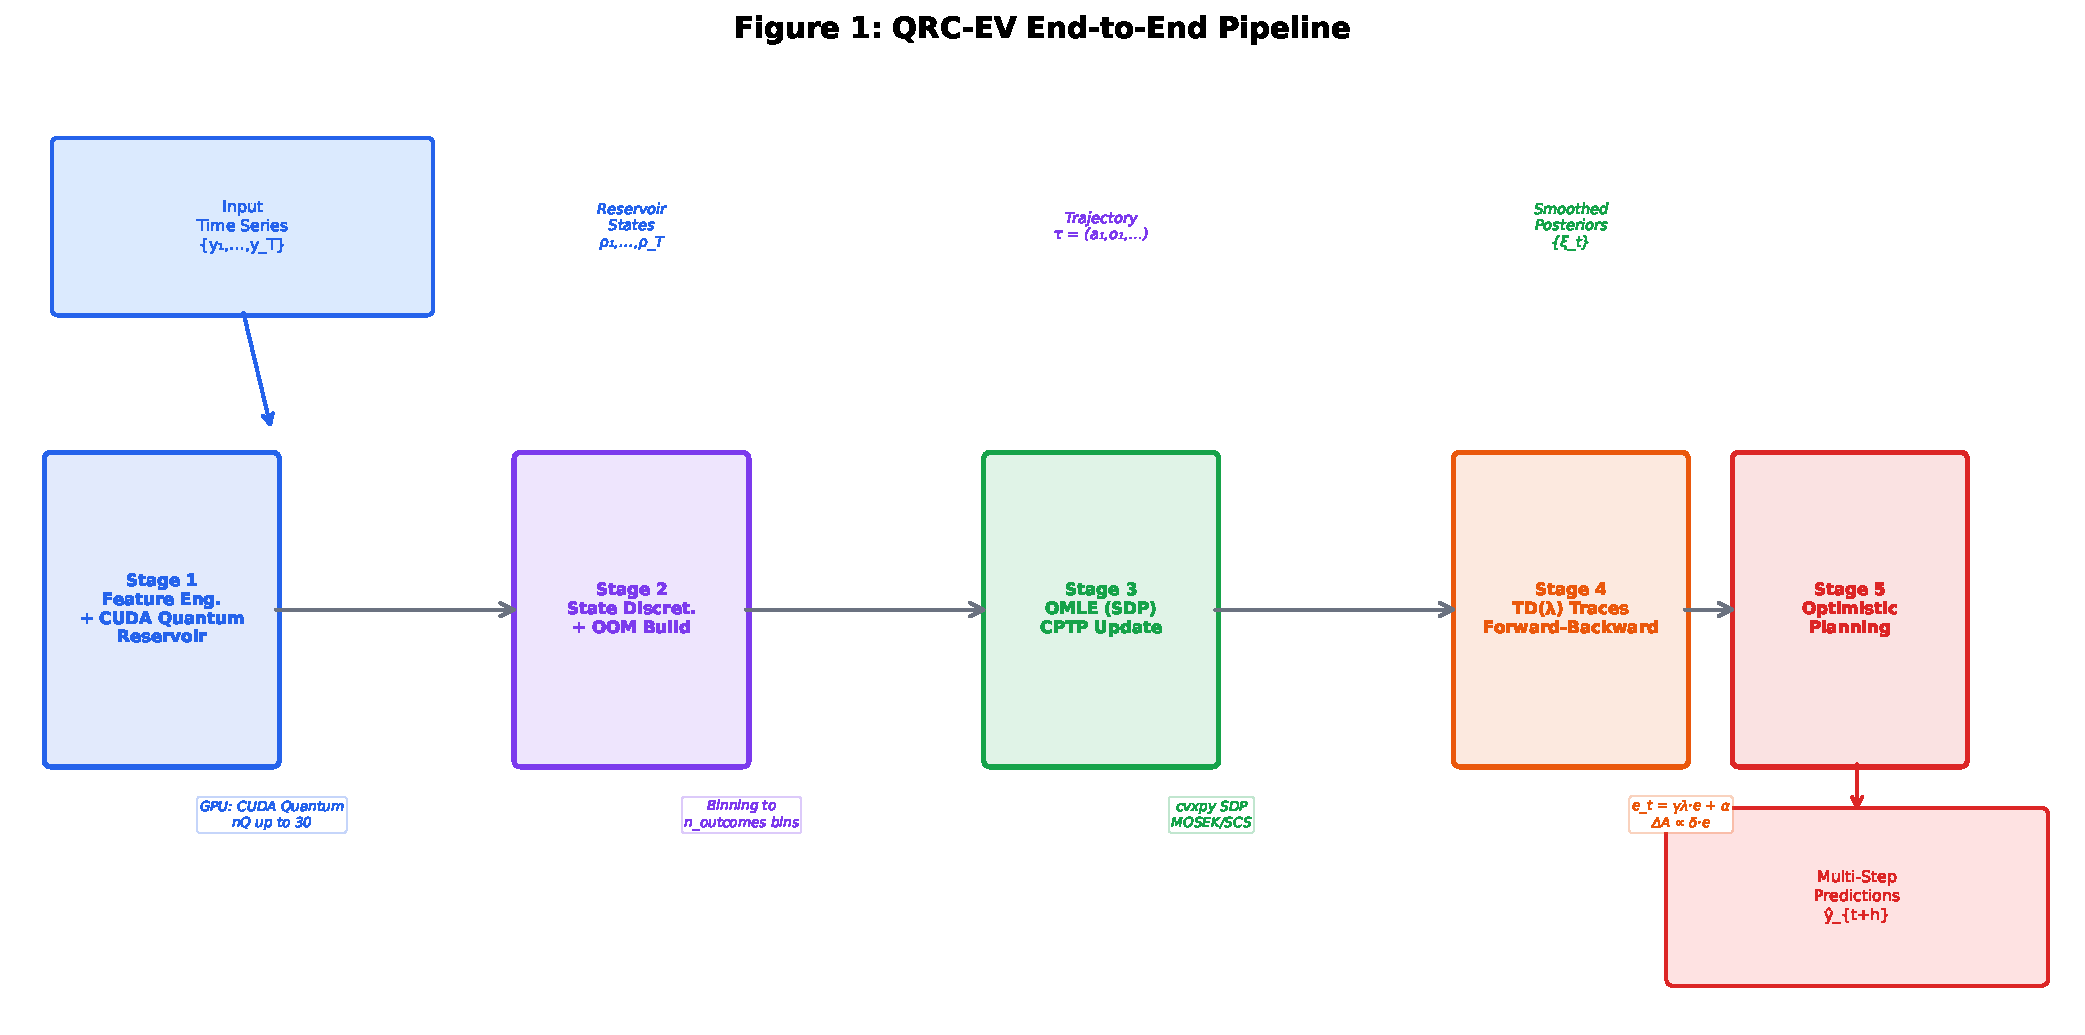
\includegraphics[width=0.95\textwidth]{figs/pipeline.pdf}
  \caption{
    QRC-EV end-to-end pipeline. (1) Input time series $\rightarrow$ feature
    engineering $\rightarrow$ CUDA Quantum reservoir (GPU). (2) Reservoir
    states $\rightarrow$ discretization $\rightarrow$ OOM transition model.
    (3) Trajectories $\rightarrow$ OMLE (SDP) $\rightarrow$ updated channels.
    (4) Forward-backward smoothing $\rightarrow$ TD($\lambda$) traces
    $\rightarrow$ parameter updates. (5) Optimistic planning $\rightarrow$
    action selection $\rightarrow$ prediction.}
  \label{fig:pipeline}
\end{figure}

\index{feature engineering}
\index{disambiguation}

The pipeline proceeds in five stages:

\index{stage 1!reservoir encoding}
\index{stage 2!disambiguation}
\index{stage 3!OMLE}
\index{stage 4!TD learning}
\index{stage 5!planning}

\subsection*{Stage 1: Feature Engineering and Reservoir Encoding}

\index{feature engineering!lagged features}
\index{rolling statistics}
Given an input time series $\{y_t\}_{t=1}^N$, we construct a lag feature
matrix:
\index{MinMaxScaler}
\begin{equation}
X[t] = \bigl[ y_{t-1}, \ldots, y_{t-n_{\mathrm{lags}}},
             \bar y_{t-n_{\mathrm{lags}}:t}, \sigma_{t-n_{\mathrm{lags}}:t},
             \sin(2\pi t / P), \cos(2\pi t / P) \bigr],
\end{equation}
where $\bar y$ and $\sigma$ are rolling mean and standard deviation over
the lag window, and $P$ is the period (e.g., $P=24$ for hourly data).
All inputs are normalized with \verb|MinMaxScaler|. The resulting feature
vector $x_t \in \mathbb{R}^{d_{\mathrm{in}}}$ is mapped to the quantum
register via the encoding map \eqref{eq:input_encoding}, and the reservoir
is evolved via \eqref{eq:reservoir_update}.

\index{periodicity!encoding}

The output at each timestep is the vectorized density matrix
$\operatorname{vec}(\rho_t) \in \mathbb{R}^{2 \cdot 2^n}$ (real and
imaginary parts concatenated), giving $d_{\mathrm{res}} = 2^{n+1}$
features per timestep.

\index{density matrix!vectorization}
\index{reservoir features!dimension}

\subsection*{Stage 2: State Discretization and OOM Model Construction}

\index{disambiguation}
\index{discretization}
\index{binning}
The continuous reservoir state $\rho_t$ must be mapped to a discrete
alphabet for the QHMM. We use a simple \textbf{binning} approach: each
timestep's reservoir features are projected to $n_{\mathrm{outcomes}}$
quantile bins, producing an outcome symbol $o_t \in \{0,\ldots,O-1\}$.
The action is set to the current lag index or a fixed default (for
purely predictive settings). This produces a discrete trajectory
$\tau = (a_1,o_1, \ldots, a_T,o_T)$.

\index{quantile binning}

The OOM transition operators $\{A^{(o,a,o',a')}\}$ are built from the
current QHMM channel and instrument estimates using the formula
\eqref{eq:oom_A_def} of Chapter~\ref{chap:background}.

\index{OOM!operator construction}

\subsection*{Stage 3: OMLE Parameter Estimation}

\index{OMLE!stage 3}
\index{SDP!stage 3}
Given a batch of trajectories, the OMLE stage solves the SDP
\eqref{eq:omle_objective} to update the channel and instrument Choi
matrices. The SDP is implemented using \verb|cvxpy| with MOSEK or SCS as
the backend. After each SDP solve, the Choi matrices are projected back
onto the CPTP constraint manifold using the trace-preserving projection.

\index{cvxpy}
\index{MOSEK}
\index{SCS}
\index{CPTP!projection}

The OMLE stage is the most computationally expensive step, requiring
$O(T \cdot S^4)$ operations per iteration for the SDP. We mitigate this
by using a small state dimension ($S=2$ for most experiments) and
limiting the number of OMLE iterations to 100.

\index{computational complexity!OMLE}

\subsection*{Stage 4: TD($\lambda$) Credit Assignment}

\index{TD($\lambda$)!stage 4}
The forward-backward algorithm is run on each trajectory to compute the
smoothed state posteriors $\{\xi_t\}$. These are used to compute the
TD error sequence $\{\delta_t\}$ using the value function
\eqref{eq:value_function}. The forward and backward traces are then
accumulated, and the combined trace is used to update the OOM transition
operators via \eqref{eq:a_update}.

\index{smoothing!stage 4}

This stage is computationally cheap: it requires only $O(T \cdot S^4)$
operations per trajectory (dominated by the forward-backward pass),
which is negligible compared to the SDP solve in Stage 3.

\index{computational complexity!TD}

\subsection*{Stage 5: Optimistic Planning and Prediction}

\index{optimistic planning!stage 5}
At inference time, the trained QHMM is used within the optimistic
planning framework to select actions that maximize expected cumulative
reward. The selected action sequence is then used to generate
multi-step predictions via the OOM forward model.

\index{multi-step prediction}
\index{horizon}

The complete prediction pipeline is:
\index{prediction!multi-step}
\begin{subequations}
\label{eq:prediction}
\begin{align}
\hat y_{t+1} &= f_{\mathrm{readout}}\bigl(\operatorname{vec}(\rho_t)\bigr), \\
\rho_{t+1} &= \mathcal{E}\bigl(U_{\mathrm{in}}(x_{t+1}) \rho_t U_{\mathrm{in}}(x_{t+1})^\dagger\bigr), \\
x_{t+1} &= \text{next input features from } \hat y_{t+1},
\end{align}
\end{subequations}
where $f_{\mathrm{readout}}$ is a Ridge regression model mapping
reservoir features to predictions.

\index{Ridge regression!readout}

The multi-step loss for horizon $h$ is
\index{loss!multi-step}
\index{NARMA}
\begin{equation}
\mathcal{L}_h = \frac{1}{N_h} \sum_{t=1}^{N_h}
  \bigl( y_{t+h} - \hat y_{t+h} \bigr)^2,
\end{equation}
where $N_h$ is the number of prediction targets at horizon $h$.
